
%%% use twocolumn and 10pt options with the asme2ej format
\documentclass[twocolumn,10pt,cleanfoot]{asme2ej}

\usepackage{graphicx} %% for loading jpg figures
\usepackage{bm}
\usepackage{nicefrac}
\usepackage{mathtools}
\usepackage{amssymb}
\usepackage{amsmath}
\usepackage{parskip}
\usepackage{listings}
\usepackage{float}
\usepackage{xcolor}

\definecolor{codegreen}{rgb}{0,0.6,0}
\definecolor{codegray}{rgb}{0.5,0.5,0.5}
\definecolor{codepurple}{rgb}{0.58,0,0.82}
\definecolor{backcolour}{rgb}{0.95,0.95,0.92}

\lstdefinestyle{mystyle}{
    backgroundcolor=\color{backcolour},
    commentstyle=\color{codegreen},
    keywordstyle=\color{magenta},
    numberstyle=\tiny\color{codegray},
    stringstyle=\color{codepurple},
    basicstyle=\ttfamily\footnotesize,
    breakatwhitespace=false,
    breaklines=true,
    captionpos=b,
    keepspaces=true,
    numbers=left,
    numbersep=5pt,
    showspaces=false,
    showstringspaces=false,
    showtabs=false,
    tabsize=2
}

\lstset{breaklines=true, style=mystyle}
%% The class has several options
%  onecolumn/twocolumn - format for one or two columns per page
%  10pt/11pt/12pt - use 10, 11, or 12 point font
%  oneside/twoside - format for oneside/twosided printing
%  final/draft - format for final/draft copy
%  cleanfoot - take out copyright info in footer leave page number
%  cleanhead - take out the conference banner on the title page
%  titlepage/notitlepage - put in titlepage or leave out titlepage
%  
%% The default is oneside, onecolumn, 10pt, final

\title{Linear regression for approximating real and synthetic data}

%%% first author
\author{Jonatan H. Hanssen
    \affiliation{
	Bachelor Student, Robotics and Intelligent Systems\\
	The faculty of Mathmatics and Natural Sciences\\
	Department of Informatics\\
    Email: jonatahh@ifi.uio.no
    }
}

\author{Eric E. Reber
    \affiliation{
	Bachelor Student, Robotics and Intelligent Systems\\
	The faculty of Mathmatics and Natural Sciences\\
	Department of Informatics\\
    Email: ericer@ifi.uio.no
    }
}


\begin{document}


\maketitle

%%%%%%%%%%%%%%%%%%%%%%%%%%%%%%%%%%%%%%%%%%%%%%%%%%%%%%%%%%%%%%%%%%%%%%
\begin{abstract}
{\it We use Ordinary Least Squares, Ridge and Lasso regression on a synthetic dataset generated by the Franke Function, and on a real dataset of elevation data from a terrain in Norway. We explore different regularization values and polynomial degrees and find that that MODEL performs best, with a MSE of NUMBER for polynomial degree 6. We find that linear regression performs well on the synthetic data, but falls short when approximating elevation data with large variances in height.
}
\end{abstract}

% \tableofcontents
% \newpage

%%%%%%%%%%%%%%%%%%%%%%%%%%%%%%%%%%%%%%%%%%%%%%%%%%%%%%%%%%%%%%%%%%%%%%
% \begin{nomenclature}
% \entry{A}{You may include nomenclature here.}
% \entry{$\alpha$}{There are two arguments for each entry of the nomemclature environment, the symbol and the definition.}
% \end{nomenclature}
%
% The primary text heading is  boldface and flushed left with the left margin.  The spacing between the  text and the heading is two line spaces.

%%%%%%%%%%%%%%%%%%%%%%%%%%%%%%%%%%%%%%%%%%%%%%%%%%%%%%%%%%%%%%%%%%%%%%
\section{Introduction}

Linear regression is a simple method in machine learning, used to create a fit of a dataset of which it can produce continuous predictions. This is achieved by assuming that we can model the output values as a linear combination of continuous functions of the input values. For example, we can assume that the observed values in our dataset can be approximated by different polynomial degrees of the input values and find the linear coefficients $\beta$ which minimize the difference between our observed and predicted values. This general idea that we can create a model which approximates our observed data with a minimal difference between observed and predicted values is a problem at the very heart of machine learning.

However, in order to create an optimal model, we require optimal parameters which cannot be known a priori. Thus, we require extensive testing and tuning of parameters to inform our selection. This presents a major obstacle, as we must for example find the optimal polynomial degree $N$ for which our model best approximates the observed values at the same time as we tune the hyperparameter $\lambda$ responsible for an adequate regularisation. We must find these parameters which lie at an intersection, where all parameters yield the minimal error in unity.

Furthermore, we will compare different models of linear regression, namely Ordinary Least Squares (OLS), Ridge and Lasso regression, and employ resampling methods, namely bootstrap and cross-validation to ensure that we draw conclusive results as these help us reduce the randomness in our parameters based off how we split our data. <source?>

%%%%%%%%%%%%%%%%%%%%%%%%%%%%%%%%%%%%%%%%%%%%%%%%%%%%%%%%%%%%%%%%%%%%%%



\section{Method}

\subsection{Theory}

This sections covers the theoretic background which underlies the methods used in this paper.

\subsubsection{Linear regression}

To describe how linear regression works, let us first describe the problem it aims to solve. Assume we have a dataset, which contains a series of inputs $\{x_i\}$, and corresponding target values $\{y_i\}$. Our assumption is that there is some relationship $y_i = f(x_i) + \epsilon_i$ where $\epsilon_i \sim N(0,\sigma^2)$, and we wish to create a model which approximates this relationship. More specifically, we wish to find a vector $\beta$ which gives us the "best" approximation $\bm{y_{pred}}$ of $\bm{y}$, by using the parameters in the following equation:

\begin{equation}
X \bm{\beta} = \bm{\tilde{y}}
\end{equation}

$X$ is called the design matrix, and is an $n$ by $p$ matrix created by our input data and our choice of basis functions, where $n$ is the amount of different input states we have (for our problem, $n$ is the number of distinct $x$ values times the number of distinct $y$ values) and $p$ is the number of features we use for our fit (in our case, $p$ is based on the polynomial degree we use). The element $X_{ij}$ is calculated by evaluating the basis function corresponding the coloumn $j$ for the input data corresponding to the row $j$. As we can see, each row of this matrix is scalar multiplied by the vector $\beta$, giving us a linear combination of the values of $X_{i*}$ for each $y_i$ in the target vector $\bm{y}$. This vector is called the parameter vector, and finding the optimal values $\hat{\bm{\beta}}$ is the problem we wish to solve. But for this, we need to define what an "optimal" prediction $\bm{\tilde{y}}$ is.

\subsubsection{The cost function}

The define the optimal prediction, we use a cost function, and the choice of cost function greatly influences what optimal parameters we get. \footnote{It is here important to keep in mind that the cost function used when fitting the model (training) rarely is the same as the one used for testing our prediction, as described in <somewhere>}. An intuitive cost function is the mean squared error (MSE). This function simply computes the average distance between our prediction and the target value, squared:

\begin{equation}
	C_{mse}(\tilde{\bm{y}}) = \sum_{i=0}^{n-1}(y_i-\tilde{y_i})^2
\end{equation}

We may now plug in the definition of $\bm{\tilde{y}}$.

\begin{equation}
	C_{mse}(\bm{\beta}) = \sum_{i=0}^{n-1}(y_i-X_{i*}\bm{\beta})^2
\end{equation}

We see that we have a function of our parameters $\bm{\beta}$, which describe how much our prediction deviates from our target values. Our problem now is to optimize this function, that is, find the values of $\beta$ which give MSE the lowest value. Luckily for us, it can be proven that the second derivative of this function is always positive (WHERE?), which means that we can find the global minimum by solving the equation

Hastie 45

\begin{gather}
\frac{\delta}{\delta \beta} \sum_{i=0}^{n-1}(y_i-X_{i*}\bm{\beta})^2 = 0 \\
 - \frac{2}{n} X^T(\bm{y} - X\bm{\beta}) = 0
\end{gather}

Solving this for $\beta$ gives us the so called normal equation, an analytical solution\footnote{This solution requires that $X^TX$ is non-singular, which may not be the case. This is solved by using the singular value decomposition of the design matrix, which we will not go into here} for the optimal $\hat{\beta}$.

% \begin{equation}
\begin{gather}
- \frac{2}{n} X^T(\bm{y} - X\bm{\beta}) = 0 \\
X^T(\bm{y} - X\bm{\beta}) = 0 \\
X^T\bm{y} - X^TX\bm{\beta} = 0 \\
X^T\bm{y} = X^TX\bm{\beta} \\
\bm{\hat{\beta}} = (X^TX)^{-1}X^T\bm{y}
\end{gather}

The process we have just described, with MSE as the cost function, is the what is known as Ordinary Least Squares (OLS) regression. Using different cost functions when fitting the model leads to different equations for $\bm{\hat{\beta}}$. This leads us to the two next forms of linear regression we use in this paper. But before this, a...

\subsubsection{Brief statistical intermission}

We must remember that our target values are defined as $y_i = f + \epsilon_i$, that is, they are distorted by a stochastic noise $\epsilon_i \sim N(0,\sigma^2)$. We should therefore take a brief intermission to prove some of the statistical qualities of the method we have just described, so as to reassure ourselves that we are justified in applying linear regression to noisy data. We will start by showing that

\begin{equation}
E[y_i] = \sum_j X_{ij}\beta_j
\end{equation}

The proof is as follows:

$\bm{y}$ is defined as the $f(\bm{x}) + \bm{\epsilon}$. We make an assumption that this can be approximated as a matrix multiplication $X\bm{\beta}$ plus an error vector $\bm{\epsilon}$. This means that each element of the vector
$\bm{y}$ can be expressed as follows:

\begin{equation}
y_i = \sum_j x_{ij}\beta_j + \epsilon_i
\end{equation}

If we take the expectation value of this expression we get the following:

\begin{gather}
E[y_i] = E\left[\sum_j x_{ij}\beta_j + \epsilon_i\right] \\
E[y_i] = E\left[\sum_j x_{ij}\beta_j\right] + E[\epsilon_i]
\end{gather}

However, the elements of $X$ are not stochastic, and neither are the elements of $\beta$ and therefore the first expectation value is simply the sum itself. Furthermore, $\epsilon$ is explicitly defined as a normal distribution $N(0,\sigma^2)$, and will by definition have the expectation value $0$. Therefore, we end up with the final expression:

\begin{equation}
E[y_i] = \sum_j x_{ij}\beta_j = \bm{X}_{i,*}\bm{\beta}
\end{equation}

Next, we show that the variance of $y_i$ is equal to the variance of the noise:

\begin{gather}
var[y_i] = E\left[(y_i - E[y_i])^2\right]  \\
= E\left[y_i^2 - 2E[y_i]y_i + E[y_i]^2\right]
\end{gather}

Distributing the outer expectation value function:

\begin{gather}
var[y_i] = E[y_i^2] - 2E\left[E[y_i]\right]E[y_i] + E\left[E[y]^2\right]  \\
= E[y_i^2] - 2E\left[E[y_i]\right]E[y_i] + E\left[E[y]\right]E\left[E[y]\right]
\end{gather}

The result of calculating the expectation value is non-stochastic. This means that $E[E[X]] = E[X]$. From this it follows that

\begin{gather}
var[y_i] = E[y_i^2] - 2E[y_i]E[y_i] + E[y_i]E[y_i]  \\
= E[y_i^2] - E[y_i]E[y_i]  \\
= E[y_i^2] - E[y_i]^2
\end{gather}

The expectation value in the second summand has been proven to be equal to $\bm{X}_{i,*}\bm{\beta}$ above. We therefore have

\begin{gather}
var[y_i] = E[y_i^2] - (\bm{X}_{i,*}\bm{\beta})^2  \\
= E\left[(X_{i,*}\bm{\beta})^2 + X_{i,*}\bm{\beta}\epsilon_i + \epsilon_i^2\right] - (\bm{X}_{i,*}\bm{\beta})^2  \\
= E\left[(X_{i,*}\bm{\beta})^2\right] + E[X_{i,*}\bm{\beta}\epsilon_i] + E[\epsilon_i^2] - (\bm{X}_{i,*}\bm{\beta})^2
\end{gather}

$X_{i,*}\bm{\beta}$ and $\epsilon_i$ are both scalars. Therefore the expectation value can be written as $E[X_{i,*}\bm{\beta}]E[\epsilon_i]$. However, $E[\epsilon_i]$ is by definition $0$, because $\epsilon_i$ is defined as a normal distribution of mean $0$ and variance $\sigma^2$. Furthermore, the expectation value of the non-stochastic $(X_{i,*}\bm{\beta})^2$ is simply the expression itself. We therefore have

\begin{gather}
var[y_i] = (X_{i,*}\bm{\beta})^2 + E[X_{i,*}\bm{\beta}]\cdot 0 + E[\epsilon_i^2] - (\bm{X}_{i,*}\bm{\beta})^2  \\
= E[\epsilon_i^2]
\end{gather}

We can prove that this is equal to the variance of $\epsilon_i$:

\begin{gather}
E[\epsilon_i^2] = \frac{1}{n} \sum_i \epsilon_i^2 \\
var[\epsilon_i] = \frac{1}{n} \sum_i (\epsilon_i - \bar{\epsilon_i})^2 \\
var[\epsilon_i] = \frac{1}{n} \sum_i (\epsilon_i - 0)^2 \\
var[\epsilon_i] = \frac{1}{n} \sum_i \epsilon_i^2 = E[\epsilon_i^2]
\end{gather}

And of course, we know that the variance of $\epsilon_i$ by definition is $\sigma^2$.

\begin{gather}
var[y_i] = E[\epsilon_i^2] = var[\epsilon_i] = \sigma^2 
\end{gather}

We should also prove some qualities about or parameters. We start by proving that $E[\hat{\beta}] = \beta$

Because we are assuming $(X^{T}X)^{-1}X^{T}$ to be deterministic, $E[(X^{T}X)^{-1}X^{T}] = (X^{T}X)^{-1}X^{T}$. Moreover, we know $E[y] = y$, and we can thus rewrite the equation as follows:

\begin{equation}
E[(X^{T}X)^{-1}X^{T}y] = (X^{T}X)^{-1}X^{T}y = \beta
\end{equation}

Next, we prove that $var(\beta) = \sigma^{2}(X^{T}X)^{-1}$.

$$var(\beta) = var((X^{T}X)^{-1}X^{T}y)$$

Because we are assuming $(X^{T}X)^{-1}X^{T}$ to be deterministic and $y$ to be stochastic, we can rewrite the $var(\beta)$ as following:

\begin{gather}
var(\beta) = (X^{T}X)^{-1}X^{T}var(y)((X^{T}X)^{-1}X^{T})^{T} \\
= (X^{T}X)^{-1}X^{T}var(y)(X^{T})^{T}((X^{T}X)^{-1})^{T}
\end{gather}

Since $(X^{T})^{T} = X$ and $(X^{T}X)^{-1})^{T}$ = $(X^{T}X)^{T})^{-1} = (X^{T}X)^{-1}$

\begin{gather}
= (X^{T}X)^{-1}X^{T}var(y)X(X^{T}X)^{-1}
\end{gather}

We know var(y) = $\sigma^{2}$, and since it is a scalar it is commutative. Thus we may move it freely

\begin{gather}
= \sigma^{2}(X^{T}X)^{-1}X^{T}X(X^{T}X)^{-1} \\
= \sigma^{2}(X^{T}X)^{-1}
\end{gather}

\subsubsection{Ridge Regression}

	A common problem with OLS is what is known as overfitting (we will discuss this in greater detail in later sections). A symptom of overfitting is that the values in the parameter vector $\bm{\beta}$ grow very large, and vary wildly for small changes in our dataset. To counteract this, we can add to the cost function a term which increases with the values in $\bm{\beta}$. Optimizing the cost function would now not only mean finding the smallest difference between target and predicted values, but also keeping the parameters small. We now define a new cost function

\begin{equation}
	C_{lasso}(\bm{\beta}) = \sum_{i=0}^{n-1}(y_i-X_{i*}\bm{\beta})^2 + \lambda \sum_{j=0}^{p-1} \beta_j^2
\end{equation}

	$||\beta||_2^2$ is equal to $\beta^T\beta$ and is simply the norm of the parameter vector, squared. With the new hyperparameter $\lambda \in (0, \inf)$ , we can decide how harshly we should punish large values in our parameter vector. Finding an optimal $\lambda$ is an important step in the process of finding the best parameters for our model.

A similar derivation as done in the previous section gives us the normal equation for Ridge regression:

\begin{equation}
	\bm{\hat{\beta}} = (X^TX + \lambda I)^{-1}X^T\bm{y}
\end{equation}

	We see that this equation, with a $\lambda > 0$ avoids the problem of an inversion of a non-singular matrix, and gives us an analytical solution for $\bm{\hat{\beta}}$ yet again. \footnote{We should cherish this analytical solution, as it may well be the last time we see a cost function that can be optimized analytically.} By using ridge regresison, we can control the complexity of our model and effectively hinder overfitting.

\subsubsection{Lasso Regression}

	Another cost function is one where we add the L1-norm (the sum of the absolute values of the parameters), instead of the L2-norm. The new cost function is as follows.

\begin{equation}
	C_{lasso}(\bm{\beta}) = \sum_{i=0}^{n-1}(y_i-X_{i*}\bm{\beta})^2 + \lambda \sum_{j=0}^{p-1} |\beta_j|
\end{equation}

However, the derivative of the absolute value is not continous, so there is sadly no analytical solution for the optimal parameters with this form of linear regression. We must then solve the problem numerically, which can be done by using Gradient Descent. Like Ridge regression, this form of regression controls the complexity of the model, with the added benifit that Lasso can drive parameters to exactly zero.

\subsubsection{Resampling methods: The bootstrap}

Bootstrap is a resampling method divided into simple steps. First, we reshuffle our dataset with replacement, which will provide us with a new dataset. Note that we will already have split our data into train and test data before we begin the bootstrap, so when we reshuffle, we will only reshuffle the training data. The reshuffled datasets act as our samples.

Secondly, we will perform our linear regression on this new dataset and store the predictions of the test data. Thirdly, we repeat for a given large number of iterations. Since we use all the test predictions to calculate the MSE, bias and variance, we will then according to the central limit theorem (REFERENCE!) obtain a normal distribution of these variables. The law of large numbers <reference?> then tells us that the mean sample values of the MSE, bias and variance approach the true value of MSE, bias and variance. This is dependent on our assumption that our data is independently and identically distributed.

These approximations of the true value of MSE, bias and variance will become useful when performing our bias-variance trade-off analysis.


\subsubsection{Cross validation}

Cross validation is another resampling technique, in which we reshuffle our data and then split them into k-folds, where k specifies the number of folds. One fold is used as our test data, and the rest is used as training data. We run our linear regression, then switch up which fold is used for testing until all folds have been used. As in bootstrapping, we will approach the true values of for example the mean squared error for our model. 
Theoretically, because both two resampling techniques use the central limit theorem and the law of large numbers, they should return the same values for the MSE, bias and variance given the same dataset. Though resampling techniques can be computationally expensive, they make up for it by aiding in model evaluation by supplying us with variables obtained from a larger number of samples. 

\subsubsection{Bias-variance trade-off}

A crucial part of model evaluation is ensuring that the model is neither underfitted nor overfitted, which we can determine by observing the relationship between the bias and the variance. Bias is defined as $(Bias[\tilde{y}])^2 = (y-E[\tilde{y}])^2$, the difference between the expected value of our prediction and the observed value. Models with high bias are usually underfitted, whilst models with low bias are the opposite. Variance on the other hand is defined as $var[\tilde{f}] = \frac{1}{n}\sum(\tilde{y_i}-E[\tilde{y}])^2$, how far away predictions are from the mean prediction. Models with high variance are usually overfitted to the training data, whilst low variance models are the opposite.

A good rule of thumb for finding a good fit is looking at the intercept between bias and variance. This is because the cost function can be decomposed into these two elements. The proof for this is as follows:

Given data $\bm{y} = f(\bm{x}) + \bm{\epsilon}$ and a OLS model $\bm{\tilde{y}} = X\bm{\beta}$, we define
the Mean Squared Error as follows

\begin{gather}
C(X,\beta) = \frac{1}{n}\sum_{i=0}^{n-1}(y_i - \tilde{y_i})^2
\end{gather}

This is simply the expectation value of $(\bm{y} - \bm{\tilde{y}})^2$

\begin{gather}
C(X,\beta) = E\left[(\bm{y} - \bm{\tilde{y}})^2\right]
\end{gather}

To derive the bias variance decomposition, we now add $E[\bm{\tilde{y}}] - E[\bm{\tilde{y}}]$ 
as a sneaky trick. We will also replace $\bm{y}$ with our definition $\bm{y} = \bm{f} + \bm{\epsilon}$

\begin{gather}
C(X,\beta) = E\left[(\bm{f} + \bm{\epsilon} - E[\bm{\tilde{y}}] + E[\bm{\tilde{y}}] - \bm{\tilde{y}})^2\right]
\end{gather}
%%%%%%%%%%%%%%%%%5
\begin{multline}
= E[(\bm{f} + \bm{\epsilon} - E[\bm{\tilde{y}}])^2 + 2[(\bm{f} + \bm{\epsilon} - E[\bm{\tilde{y}}])(E[\bm{\tilde{y}}] \\
	- \bm{\tilde{y}})] +(E[\bm{\tilde{y}}] - \bm{\tilde{y}})^2]
\end{multline}

\begin{multline}
= E[(\bm{f} + \bm{\epsilon} - E[\bm{\tilde{y}}])^2] + \\
	2E[(\bm{f} + \bm{\epsilon} - E[\bm{\tilde{y}}])(E[\bm{\tilde{y}}] - \bm{\tilde{y}})] + E[(E[\bm{\tilde{y}}] - \bm{\tilde{y}})^2]
\end{multline}

Let us focus our attention on the middle term first.

\begin{gather}
2E\left[(\bm{f} + \bm{\epsilon} + E[\bm{\tilde{y}}])(E[\bm{\tilde{y}}] - \bm{\tilde{y}})\right] 
\end{gather}

Expanding the multiplication:

\begin{gather}
2E\left[\bm{f}E[\bm{\tilde{y}}] + \bm{\epsilon}E[\bm{\tilde{y}}] - E[\bm{\tilde{y}}]E[\bm{\tilde{y}}] - \bm{f}\bm{\tilde{y}} - \bm{\epsilon}\bm{\tilde{y}} + E[\bm{\tilde{y}}]\bm{\tilde{y}}\right] 
\end{gather}

Distributing the expectation value:

\begin{gather}
2\left[E[\bm{f}E[\bm{\tilde{y}}]] + E[\bm{\epsilon}E[\bm{\tilde{y}}]] - E[E[\bm{\tilde{y}}]E[\bm{\tilde{y}}]] - E[\bm{f}\bm{\tilde{y}}] - E[\bm{\epsilon}\bm{\tilde{y}}] + E[E[\bm{\tilde{y}}]\bm{\tilde{y}}]\right] 
\end{gather}

We know that $\bm{\tilde{y}}$ and $\bm{f}$ are non-stochastic, and we know that the expectation value of $\bm{\epsilon}$ is $0$. We also know that 
$\bm{\epsilon}$ and $\bm{\tilde{y}}$ are independent, which means we can write $E[\bm{\epsilon}\bm{\tilde{y}}]$ as $E[\bm{\epsilon}]E[\bm{\tilde{y}}]$ We therefore have

\begin{gather}
2\left[\bm{f}\bm{\tilde{y}} + 0 - \bm{\tilde{y}}\bm{\tilde{y}} - \bm{f}\bm{\tilde{y}} - 0 + \bm{\tilde{y}}\bm{\tilde{y}}\right] = 0 
\end{gather}

We then have

\begin{gather}
C(X,\beta) = E\left[(\bm{f} + \bm{\epsilon} - E[\bm{\tilde{y}}])^2\right] + E\left[(E[\bm{\tilde{y}}] - \bm{\tilde{y}})^2\right] 
\end{gather}

The second term is by definition the variance of model.

\begin{gather}
C(X,\beta) = E\left[(\bm{f} + \bm{\epsilon} - E[\bm{\tilde{y}}])^2\right] + var[\bm{\tilde{f}}] 
\end{gather}

And now the final term

\begin{gather}
E\left[(\bm{f} + \bm{\epsilon} - E[\bm{\tilde{y}}])^2\right]
\end{gather}

\begin{multline}
= E[\bm{f}^2 + \bm{f}\bm{\epsilon} - \bm{f}E[\bm{\tilde{y}}] + \bm{f\epsilon} + \bm{\epsilon}^2 - \\ 
	\bm{\epsilon}E[\bm{\tilde{y}}] - \bm{f}E[\bm{\tilde{y}}] - \bm{\epsilon}E[\bm{\tilde{y}}] + E[\bm{\tilde{y}}]^2]
\end{multline}

After distributing the expectation value we get the following, keeping in mind that $E[\bm{f}] = E[\bm{y} - \bm{\epsilon}] = E[\bm{y}] - E[\bm{\epsilon}] = \bm{y}$

\begin{gather}
\bm{y}^2 - 2\bm{y}\bm{\tilde{y}} + E[\bm{\tilde{y}}]^2 + \sigma^2 \\
(\bm{y} + E[\bm{\tilde{y}}]^2 + \sigma^2 
\end{gather}

We see that the quadratic form is equal to $bias[\bm{\tilde{y}}]^2$. We can then conclude that the cost function can be rewritten as follows:

\begin{gather}
C(X,\beta) = bias[\bm{\tilde{y}}]^2 + var[\bm{\tilde{f}}] + \sigma^2 
\end{gather}


Because the cost function is a sum of the bias and the variance, the lowest error will generally occur when both bias and variance are low. This also fits our understanding of the definitions of bias and variance, as we wish to obtain a model that is neither high in bias (underfitted) or high in variance (overfitted).


With the theory explained, we can go on to describe how we have applied it to our problem.


%%%%%%%%%%%%%%%%%%%%%%%%%%%%%%%%%%%%%%%%%%%%%%%%%%%%%%%%%%%%%%%%%%%%%%


\subsection{Implementation}
\subsubsection{Preprocessing: Creating the design matrix and normalizing our data}
We have two datasets, one synthetic and one real. Regardless of the source of the data, we create the design matrix in a similar manner, as the relation between our input data and our target values are the same for both datasets, that is, for each combination of $x$ and $y$, we have a height $z$. For the Franke function this height is no more than the height over the $xy$-plane, but for our real data, this value represents the elevation in meters above ocean level for a terrain in Norway. As we want to do a polynomial fit of the data, we create our design matrix such that each row $i$ has the following values:

\begin{equation}
X_{i*} = 1 \;\; x_i \;\; y_i \; x_i^2 \;\; x_i y_i \;\; y_i^2 \;\; ... \;\; x_i^p y_i^p
\end{equation}

	Below is the python code used to create the design matrix, which can be found in \texttt{src/utils.py}.

\lstinputlisting[language=Python, firstline=27, lastline=42]{../../src/utils.py}

	While the creating of the design matrix is equivalent for the two datasets, the preprocessing of the data afterwards is not. For the Franke function, we claim that no normalization is needed, as we generate the data ourselves to be between $0$ and $1$. Given that we are doing a polynomial fit, every element in our design matrix will be a multiplication of $x^p$ and $y^k$ for different $p$'s and $k$'s, which, given our choice of range for $x$ and $y$, guarantees that every element is between $0$ and $1$. However, we have included a centering of the data, which has no effect on the Ordinary Least Squares regression, but which is used when applying Ridge and Lasso regression, to avoid punishing the intercept. The centering is done as follows: First, the first coloumn of the design matrix (the intercept coloumn) is discarderd. Then we calculate the mean for the target values and the design matrix (the mean for the design matrix is a vector with mean values for each coloumn). We subtract this from the design matrix and target values when performing the fit giving us a vector $\bm{\beta}$. Afterwards we calculate the intercept with the following equation

\begin{equation}
	intercept = mean(\bar{y} - \bar{X}_c^T \bm{\beta})
\end{equation}

	where $\bar{y}$ is the mean value of $\bm{y}$ and $\bm{\bar{X}_c}$ is a vector of size $p$ with $\bar{X}_i = mean(X_i)$ (the mean of each coloumn in $X$). We finally create our prediction by using the $\bm{\beta}$, $X$ and intercept we calculated above:

\begin{equation}
	\bm{\hat{y}} = X \bm{\beta} + intercept
\end{equation}

The code for this, taken from the \texttt{evaluate\_model} function in \texttt{src/utils.py} is as follows: \footnote{Some intermediate parts of our implementation not related to this have been removed for readability}

\begin{lstlisting}[language=Python]
X_train = X_train[:, 1:]
z_train_mean = np.mean(z_train, axis=0)
X_train_mean = np.mean(X_train, axis=0)
beta = model((X_train - X_train_mean), (z_train - z_train_mean))
intercept = np.mean(z_train_mean - X_train_mean @ beta)
z_pred_train = X_train @ beta + intercept
\end{lstlisting}

Where \texttt{model} calculates \texttt{beta} using the normal equations for OLS.

For the real elevation data, normalization is definitely required, as the values for $x$, $y$ reach several hundred and $z$ reaches over a thousand. For polynomial degree $10$ and an $x$ value which reaches $400$, we will have a design matrix with values from $0$ to $400^{10}$. This large range of values makes our linear regression perform poorly (WHY?). We have therefore chosen to scale our design matrix using Scikit's \texttt{MinMaxScaler}, which scales each column to be in the range of $(0,1)$. The calculation of mean and variance is done on the training data, and applied to both the training and test data. We have done the same with the values for $z$. This gives a much more stable model. The code for doing this on the design matrix is as follows, taken from \texttt{src/utils.py}:

\lstinputlisting[language=Python, firstline=238, lastline=245]{../../src/utils.py}

Another form of "preprocessing" which is strictly practical in nature, is that we have reduced the dimensions of the data to 320 by 640. This was done by downscaling the image. \footnote{The interpolation was done using "nearest neighbor interpolation", which does not introduce new values into the data. An equivalent programmatic solution would be to for instance only look at every 4 pixels} This was simply done because the design matrix becomes several gigabytes in size if one uses the whole dataset, and model fitting takes an unreasonable amount of time.

%%%%%%%%%%%%%%%%%%%%%%%%%%%%%%%%%%%%%%%%%%%%%%%%%%%%%%%%%%%%%%%%%%%%%%

\subsubsection{Implementation of linear regression}

Linear regression for OLS and Ridge are implemented by using NumPy's \texttt{numpy.linalg.pinv} and the normal equations. We have implemented them as functions which take in the target values and the design matrix and return $\bm{\hat{\beta}}$. They are called from a wrapper function called \texttt{evaluate\_model} which takes care of the scaling and works with both SciKit models and our own. Below are the functions, taken from \texttt{src/utils.py}:

\lstinputlisting[language=Python, firstline=53, lastline=64]{../../src/utils.py}

For repeated calls of these functions with different polynomial degrees, we use the function \texttt{linreg\_to\_N}, which passes the correctly sliced design matrix to the regression functions and saves the predictions and various performance metrics for each polynomial degree for easy plotting.

For Lasso regression, we use SciKit's implementation. We also use SciKit's implementation for OLS and Ridge for comparisons with our own implementation.

\subsubsection{Implementation of resampling methods}

We use resampling methods to better estimate our performance metrics. We use both cross validation and the bootstrap method. Cross validation is implemented in the function \texttt{crossval} in \texttt{src/utils.py}. We split the data into $K$ folds by slicing with NumPy taking consecutive rows of the design matrix and target vector. But before we do this, we resample the data with Scikit's \texttt{resample}. This is important because our $x$'s and $y$'s are not normal distributions but consecutive values between $0$ and $1$, and therefore consecutive rows correspond specific areas of our data, which is not wanted. We then fit on $K-1$ folds, and test on the last. We return the average error.

We implement bootstrap by repeatedly resampling our data with replacement and performing the prediction. We use the predictions returned from hundreds of resamplings to calculate the bias and variance of our model.

\subsubsection{Franke Function}

We use the Franke Function with an added stochastic noise of to test our models. We explore how higher and lower levels of noise affect the model. Below is the Franke function:

\begin{multline}
f(x,y) = \frac{3}{4}\exp{\left(-\frac{(9x-2)^2}{4}-\frac{(9y-2)^2}{4}\right)} + \\ \frac{3}{4}\exp{\left(-\frac{(9x+1)^2}{49}-\frac{(9y+1)}{10}\right)} + \\
\frac{1}{2}\exp{\left(-\frac{(9x-7)^2}{4}-\frac{(9y-3)^2}{4}\right)} - \\
\frac{1}{5}\exp{\left(-(9x-4)^2-(9y-7)^2\right)}
\end{multline}

As we can see, it is simply a weighted sum of exponentials. As such it has an infinite Taylor expansion into polynomials.\footnote{The proof for this is left as an exercise for the reader}


\section{Results}

\subsection{Franke Function}

To gain insight into how the three different regression methods work, we experiment with synthetic data generated by the Franke function.

\subsubsection{Ordinary Least Squares}

%%%%%%% FIGURES %%%%%%%%%
\begin{figure*} 
\centerline{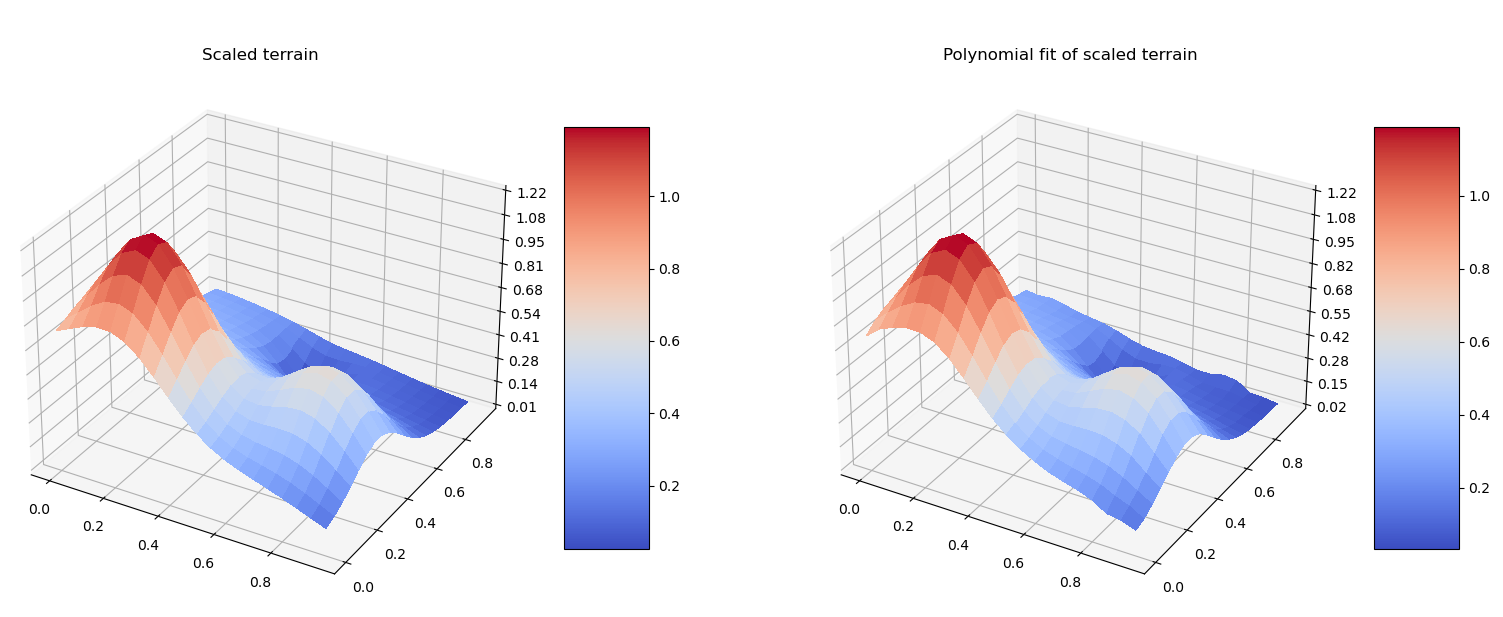
\includegraphics[width=6.85in]{figure/frankenonoise.png}}
\caption{A comparison of our best OLS prediction and the Franke function with no noise, at polynomial degree 10}
\label{frankenonoise}
\end{figure*}

\begin{figure} 
\centerline{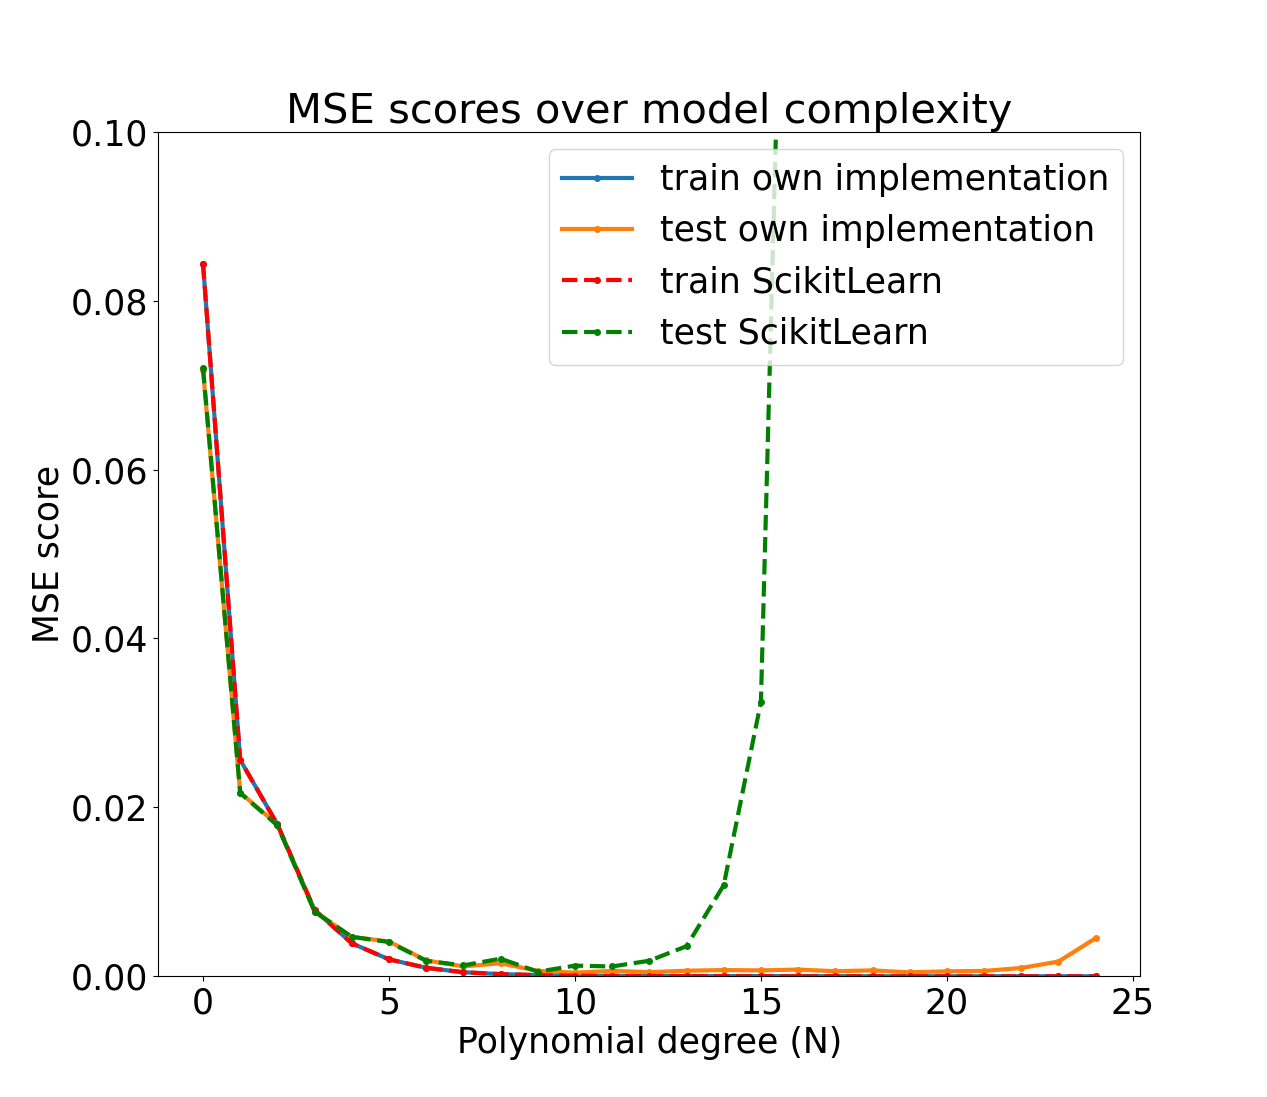
\includegraphics[width=3.25in]{figure/frankenonoisemse.png}}
\caption{Test and train MSE for the Franke function with no noise, using OLS}
\label{frankenonoisemse}
\end{figure}

We find that OLS creates a good fit for the Franke Function. With 400 datapoints, we can increase our polynomial degree to around 20 before we see signs of overfitting.\footnote{Here we also see something a bit surprising: We see that our own implementation of OLS follows Scikit's implementation up to around polynomial degree 10, at which point scikit's MSE increases rapidly. We chalk this up to numerical errors and differing implementation of the normal equations, as we simply use the normal equation exactly, while scikit uses an implementation which is probably computationally more efficient but gives slight differences when comparing to the normal equation. These differences seem to create a large error after a certain size of the design matrix is reached, which we can not adequately explain.} This is most likely because the Franke function can be expanded into a sum of polynomials. We would expect to see higher polynomial degrees give us better and better prediction, up to a certain point.\footnote{And indeed, this seems to be the case, as if we increase the availiable datapoints considerably, as seen in Fig.~\ref{frankiehigherdatapoints} in the appendix, we can reach much higher polynomial degrees without overfitting} When we reach degrees higher than around 20, we see that our test error increases slightly, a sign of overfitting. This is also to be expected, as even if the continual Franke function could be expanded into a series of polynomials, we are working with a limited dataset of only 400 samples (and only 320 of those in our training set). As we reach higher and higher degrees, we are more and more likely to see unlucky train-test-splits where the best fit for the training data leads to large errors for the test data. See Fig.~\ref{frankenonoise} for a comparison between the Franke function and our best prediction, which shows that they are essentially identical. Fig.~\ref{frankenonoisemse} shows the train and test MSE by polynomial degree. The MSE for test in these plots is the average MSE for 100 bootstraps. For a full list of all parameters used for every plot shown, see Table.~\ref{allparamstable} in the appendix.

However, when we introduce a stochastic noise, we see that overfitting happens rapidly. Without a regularization hyperparameter, parameters fluctuate wildly and our prediction suffers. Fig.~\ref{frankenoisemse} shows our MSE up to polynomial degree 25 with an added stochastic noise $\epsilon \sim N(0,0.05)$, where we see that we are overfitting severely. See Fig.~\ref{frankienoisecomparison} in the appendix for test MSE for more and more noisy target values. 

\begin{figure} 
\centerline{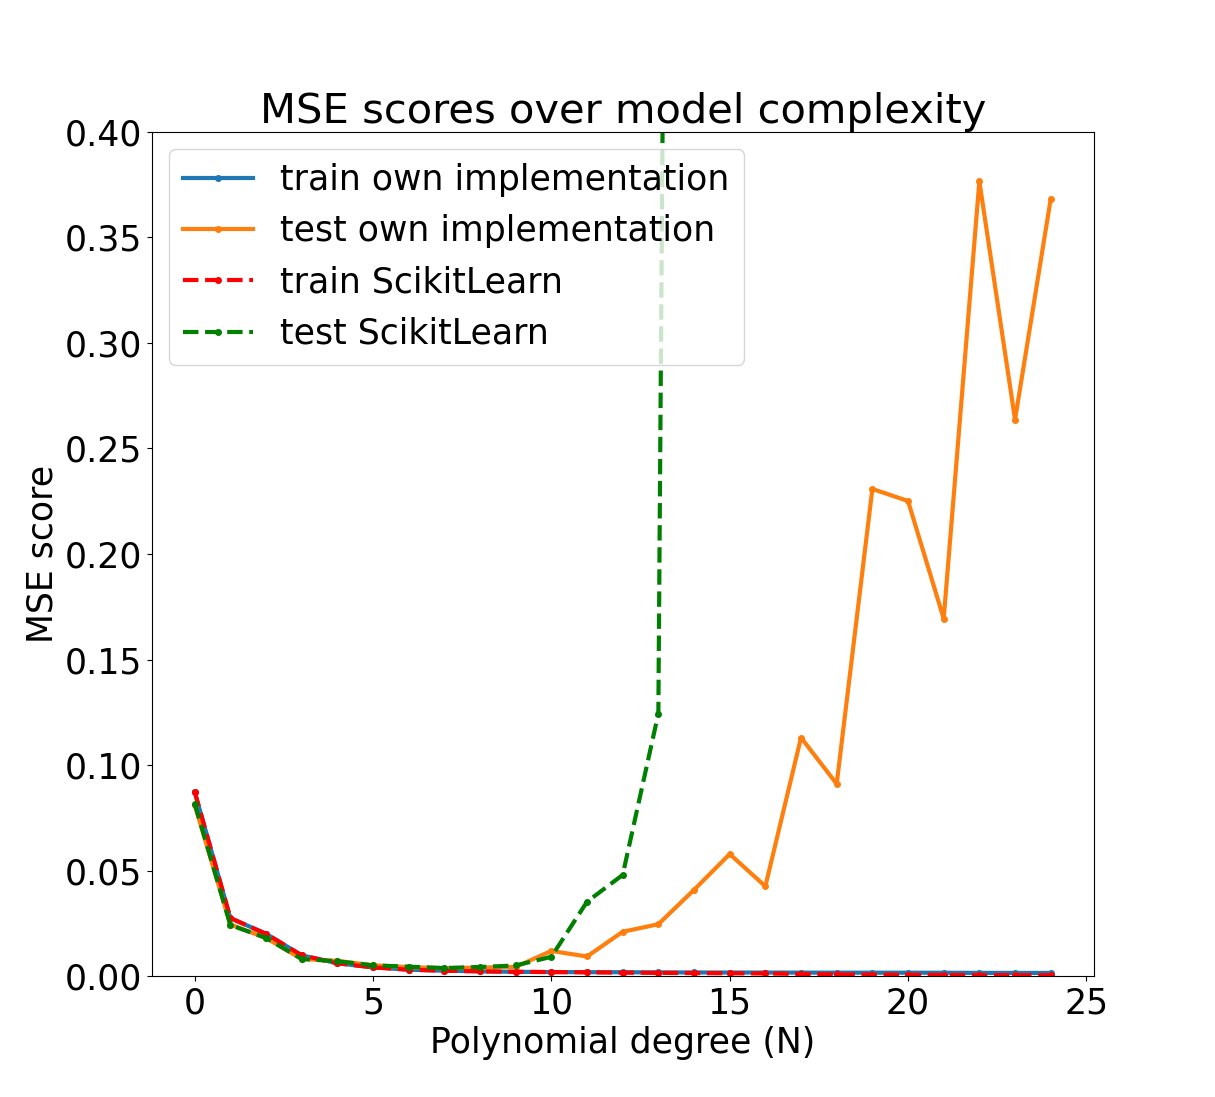
\includegraphics[width=3.25in]{figure/frankenoisemse.png}}
\caption{Test and train MSE for the Franke function with noise, using OLS}
\label{frankenoisemse}
\end{figure}

By using bootstrap resampling, we can study the bias-variance-tradeoff, which shows how the variance of our model between different bootstraps iterations increases as our model overfits our noisy data. See Fig.~\ref{frankiebiasvariance}. Clearly, we need to introduce regularization if we want a model that does not overfit. Fig. ~\ref{frankenoisybeta} in the appendix shows the beta progression for selected betas, clearly showing that we are overfitting.

\begin{figure} 
\centerline{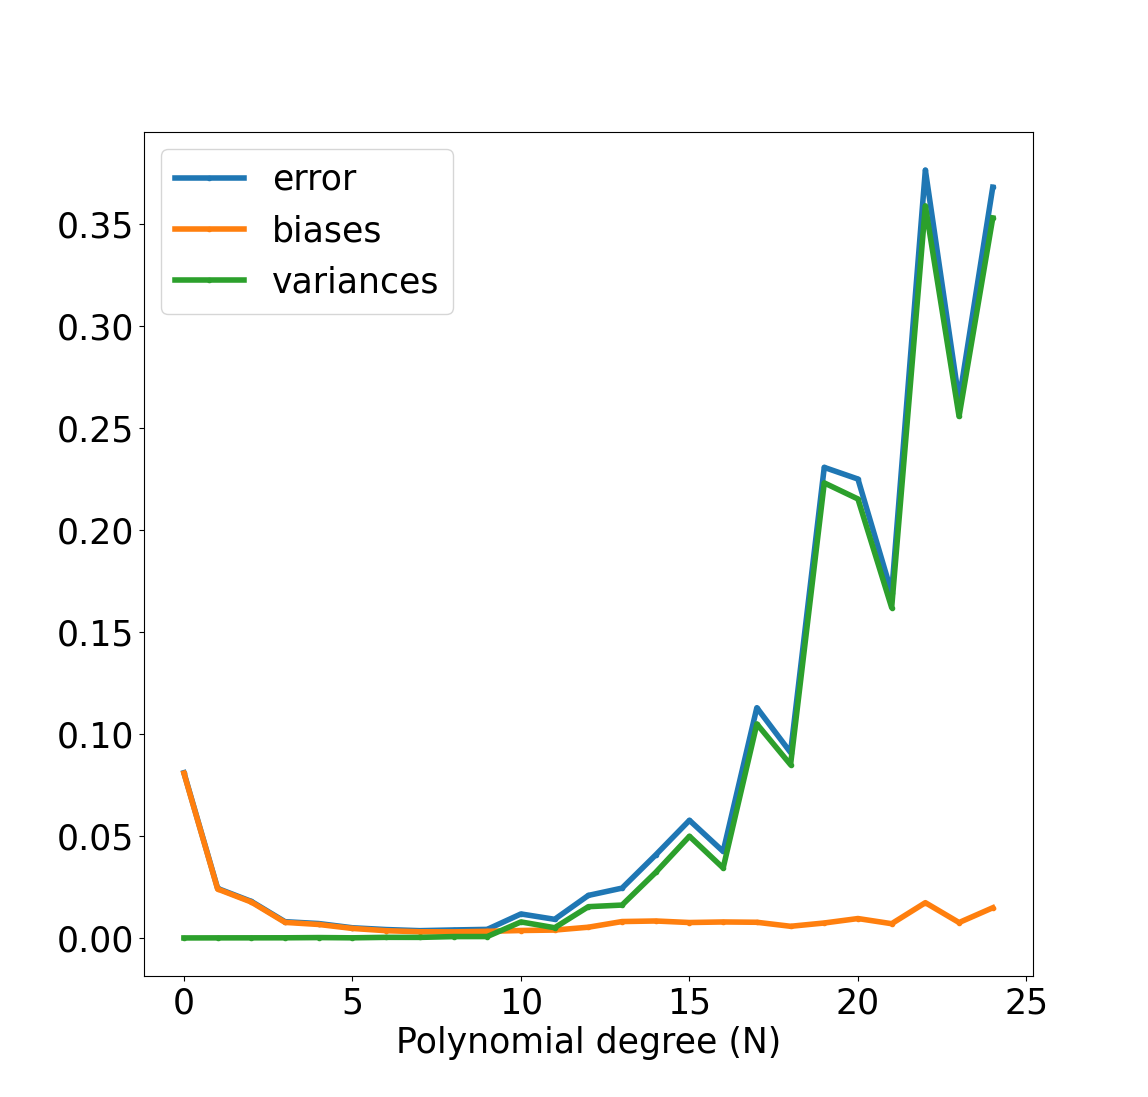
\includegraphics[width=3.25in]{figure/frankiebiasvariance.png}}
\caption{Bias, variance and test MSE plotted over polynomial degree for our OLS prediction on the Franke function with an added stochastic noise $\epsilon \sim N(0,0.05)$}
\label{frankiebiasvariance}
\end{figure}

Table. ~\ref{ols_mse_table} shows the best polynomial degree and MSE for regular and noisy data. Here we see that the best degree without noise is 10, which shows that even without noise, the low amount of data leads to a slight overfit even at very small polynomial degrees. This is not surprising, as at $N = 10$ we have $66$ features, which is a substantial amount compared to our measly 320 training datapoints. We could of course arbitrarily increase our dataset to ludicrous levels, but doing linear regression with this dataset gives valuable insight into how our performance is dependent on our availiable data.

\begin{table}[t]
\caption{Best MSE and polynomial degree for OLS}
\begin{center}
\label{ols_mse_table}
\begin{tabular}{c l l}
% & & \\ % put some space after the caption
% \hline
Std of noise & Best MSE & Best degree \\
\hline
0 & 0.0004335 & 10\\
0.05 & 0.0038302 & 7 \\
0.10 & 0.0139833 & 7 \\
\hline
\end{tabular}
\end{center}
\end{table}

\subsubsection{Ridge}

Using Ridge regression, we see from Fig.~\ref{frankiedifflambdas} that larger and larger values of $\lambda$ efficiently prevents overfitting and reduces the variance between predictions. Looking at the beta progression with for the same values of $\lambda$ (Fig.~\ref{frankeridgebetas}), we see that the regularization parameter is successfully shrinking the beta values. Using Scikit's gridsearch, we find the optimal $\lambda$ to be $10^{-8}$ and the optimal polynomial degree to be 7, with an average MSE of $0.0037999$, which is very slightly lower than OLS for the Franke function with an added stochastic noise $\epsilon \sim N(0,0.05)$. We see from this that Ridge regression has not really had much of an effect in decreasing the MSE. We must now remember what Ridge aims to do. With the regularization parameter, we can prevent overfitting if our model is too complex for our data. But we should recall that we decide the complexity of our model, by deciding which polynomial degree we use when creating the design matrix. In fact, by choosing polynomial degree 7 for our OLS method to get the best MSE for noisy data, we are in fact doing a primitive form of best subset selection, as described in Hastie et Al. p 57 \cite{hastie}. Almost by definition, the polynomial degree with the best MSE is not overfitted, because if it was, it would not be the model with the lowest MSE among all polynomial degrees. Therefore it is not so unexpected that Ridge regression has a relatively low impact on the MSE. We could expect that Ridge would allow us to reach higher polynomial degrees without overfitting, by shrinking features of the higher polynomial degrees that are not supported but allowing us to keep other high degree terms (for example, allowing us to use $x^5y^4$, but discard $x^9$, if only $x^5y^4$ was supported by the data). But we can see from the Table. ~\ref{ols_vs_ridge_table} that we are not able to push into higher degrees. A possible explanation for this is that every feature is useful, due to the polynomial expansion of the Franke function. 


\subsubsection{Lasso}

Looking at Lasso regression, we find that it has the same capability to reduce overfitting as Ridge, as can be seen in Fig.~\ref{frankelassodifflambdas}.

\begin{table}[t]
\caption{Best MSE for Ridge regression and OLS with 400 datapoints}
\begin{center}
\label{ols_vs_ridge_table}
\begin{tabular}{c | l l l}
% & & \\ % put some space after the caption
% \hline
Regression & Std of noise & Best MSE & Best degree \\
\hline
OLS & 0.05 & 0.0038302 & 7 \\
Ridge & 0.05 & 0.0037999 & 7 \\
\hline
\end{tabular}
\end{center}
\end{table}

\begin{figure} 
\centerline{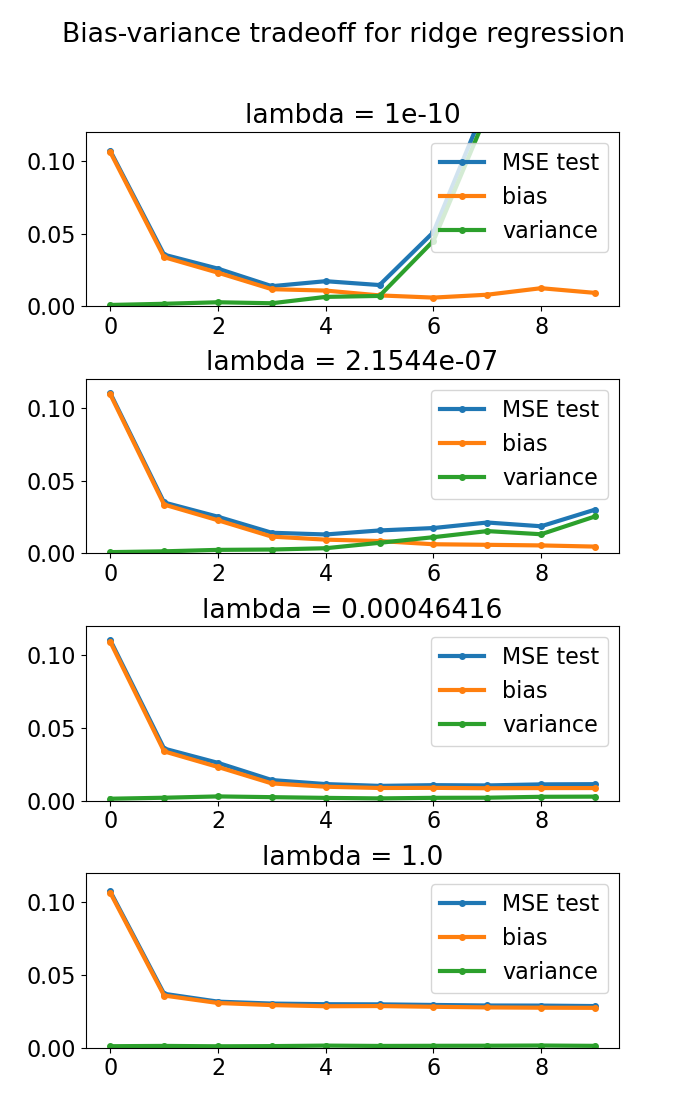
\includegraphics[width=3.25in]{figure/frankiedifflambdas.png}}
\caption{Bias, variance and test MSE plotted over polynomial degree for our Ridge prediction on the Franke function with an added stochastic noise $\epsilon \sim N(0,0.05)$, using lambdas of increasing size. Here we have reduced the number of datapoints to only 100 to force overfitting earlier.}
\label{frankiedifflambdas}
\end{figure}

\subsubsection{Lasso}

Turning our attention to Lasso regression, we also find that overfitting can be avoided with a good choice of $\lambda$. Comparing the three methods, we see that for noisy target data, Ridge and Lasso are superior to OLS, as seen in Fig. NUMBER.

\subsection{Elevation data}

With the confidence that our methods work as expected on synthetic data, we turn our attention to the real elevation data. 

\subsubsection{Ordinary Least Squares}

Here we find some limitations of linear regression. We see from Fig. NUMBER that the we are able to fit the terrain up to a certain point, gaining an MSE of NUMBER with OLS with polynomial degree DEGREE. However, we see that beyond this, we have little to gain. This can be seen when we increase the polynomial degree to very large amounts, without seeing any decrease in MSE (Fig. NUMBER). Looking at the beta progression for selected betas (Fig. NUMBER), we see that the parameters stabilize, which implies that we are not overfitting, but simply reaching our best possible prediction for polynomial regression. The fact that we are not overfitting is further reinforced by looking at the bias-variance plot in Fig. NUMBER, which shows no increase in variance. It is reasonable to expect that our model will not overfit, due to the large increase in data we now use for the fit. Our synthetic data used $20 x 20 = 400$ datapoints, while we now have $320 x 640 = 204 800$ datapoints. This means that for a 50th order polynomial, which will have $1326$ features, our number of features are less than $1\%$ of our datapoints. If we decrease the number of datapoints used for training considerably, we can see overfitting start to occur (see Appendix 1). So we are not overfitting, but we are not decreasing our MSE either. This is likely because the elevation data has a jagged and complex shape, which cannot be accurately recreated, even with a polynomial of degree $50$. We should remember that the Franke function can be expanded into a series of polynomials, which is why we can expect to get a lower and lower MSE as the polynomial degree increases (so long as we have enough data and it is not noisy). The same is not true for our elevation data, and as such we have little to gain from increasing our model complexity after a certain point. Clearly, linear regression does not offer a very good tradeoff between computational cost and performance for this data.

\subsubsection{Ridge Regression}

As our model is not overfitting, we do not expect Ridge to offer much improvement. 

%%%%%%%%%%%%%%%%%%%%%%%%%%%%%%%%%%%%%%%%%%%%%%%%%%%%%%%%%%%%%%%%%%%%%%
%%%%%%%%%%%%%%%% begin figure %%%%%%%%%%%%%%%%%%%
% \begin{figure}[t]
% \begin{center}
% \setlength{\unitlength}{0.012500in}%
% \begin{picture}(115,35)(255,545)
% \thicklines
% \put(255,545){\framebox(115,35){}}
% \put(275,560){Beautiful Figure}
% \end{picture}
% \end{center}
% \caption{The caption of a single sentence does not have period at the end}
% \label{figure_ASME} 
% \end{figure}
%%%%%%%%%%%%%%%% end figure %%%%%%%%%%%%%%%%%%% 
%%%%%%%%%%%%%%%%%%%%%%%%%%%%%%%%%%%%%%%%%%%%%%%%%%%%%%%%%%%%%%%%%%%%%%



%%%%%%%%%%%%%%%% begin figure %%%%%%%%%%%%%%%%%%%
% \begin{figure} 
% \centerline{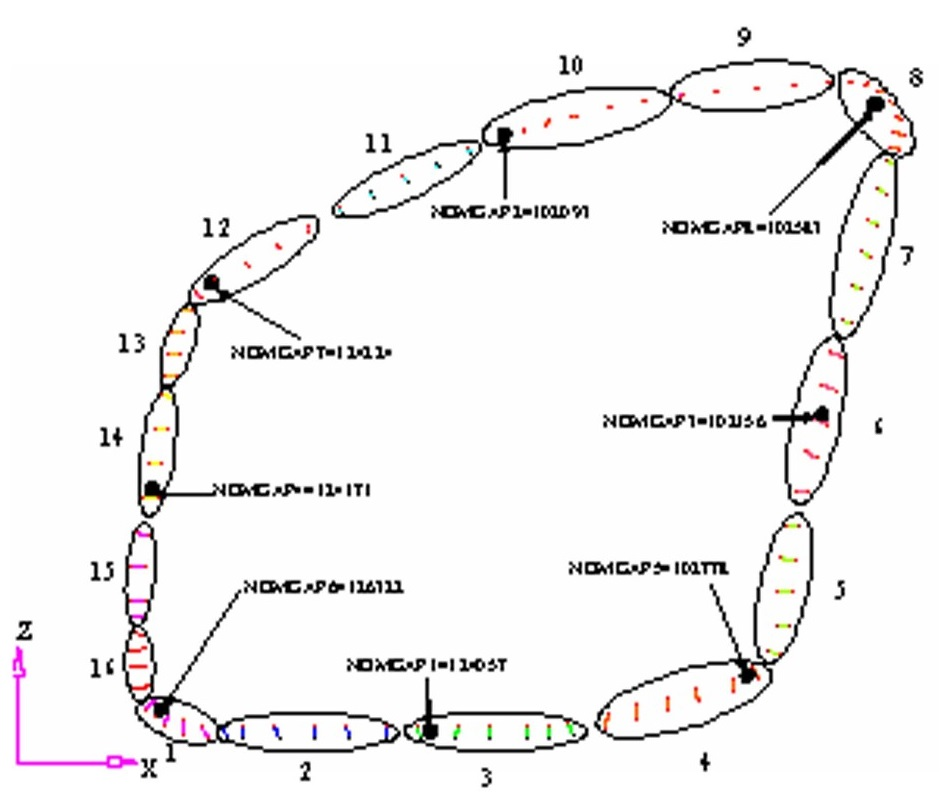
\includegraphics[width=3.34in]{figure/FMANU_MD_05_1272_5.jpg}}
% \caption{While this figures is easily readable at a double column width of 6.5in, when it is shrunk to 3.25in column width the text is unreadable. This paper was held from production.}
% \label{fig_example2.jpg}
% \end{figure}
%%%%%%%%%%%%%%%% end figure %%%%%%%%%%%%%%%%%%%

%%%%%%%%%%%%%%%% begin figure %%%%%%%%%%%%%%%%%%%
%%% the maximum width in double column is 6.85in
% \begin{figure*} 
% \centerline{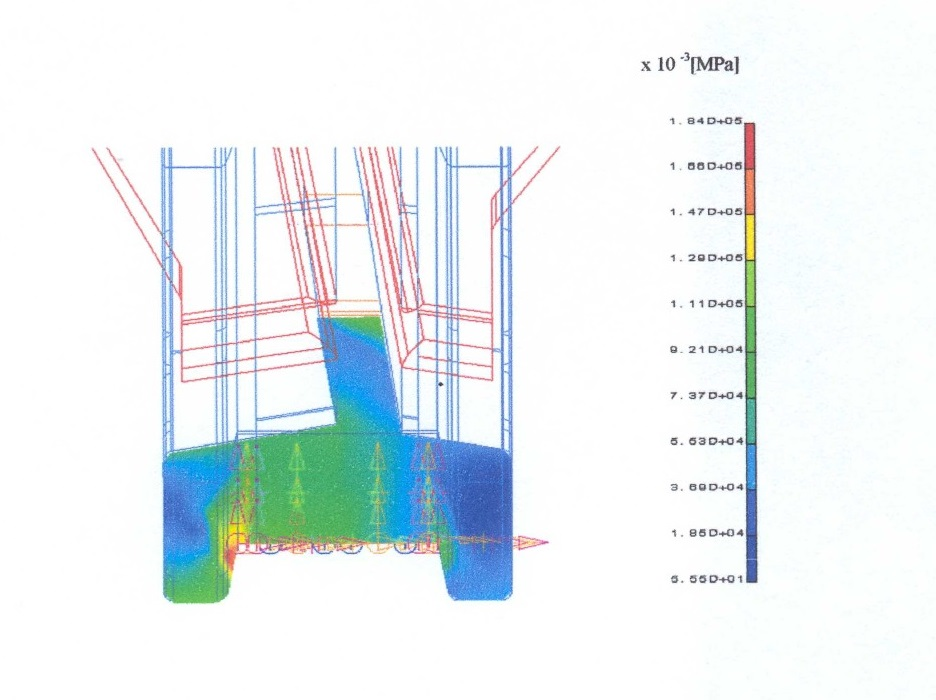
\includegraphics[width=6.85in]{figure/FMANU_MD_04_1274_13.jpg}}
% \caption{A figure expanded to double column width the text from Figure~\ref{fig_example3.jpg}}
% \label{fig_example4.jpg}
% \end{figure*}
%%%%%%%%%%%%%%%% end figure %%%%%%%%%%%%%%%%%%%
%%%%%%%%%%%%%%%%%%%%%%%%%%%%%%%%%%%%%%%%%%%%%%%%%%%%%%%%%%%%%%%%%%%%%%


\bibliographystyle{alpha}
\bibliography{bibliography}

%%%%%%%%%%%%%%%%%%%%%%%%%%%%%%%%%%%%%%%%%%%%%%%%%%%%%%%%%%%%%%%%%%%%%%
\appendix       %%% starting appendix
\section*{Appendix A: Plots and tables}

The next pages contain plots and tables that are of interest.



\begin{table*}
\caption{This table shows every applicable parameter for every figure, so that they may be easily reproduced. Every plot uses the random seed 42069}
\begin{center}
\label{allparamstable}
\begin{tabular}{c | l l l l l l l}
% & & \\ % put some space after the caption
% \hline
Figure & Highest $N$ & Std of noise & Number of datapoints & Bootstraps & K-folds & $\lambda$ & Scaling \\
\hline
\ref{frankenonoise} & 10 & 0 & 400 & - & - & - & None\\
\ref{frankenonoisemse} & 25 & 0 & 400 & 100 & - & - & None\\
\ref{frankenoisemse} & 25 & 0.05 & 400 & 100 & - & - & None\\
\ref{frankiebiasvariance} & 25 & 0.05 & 100 & 100 & - & - & None\\
\ref{frankiedifflambdas} & 25 & 0.05 & 100 & 100 & - & variable & Centering\\
\ref{frankienoisecomparison} & 25 & variable & 400 & 100 & - & - & None\\
\ref{frankiehigherdatapoints} & 30 & 0 & 10000 & 100 & - & - & None\\
\hline
\end{tabular}
\end{center}
\end{table*}

\begin{figure*}
% \begin{figure}[t]
\centerline{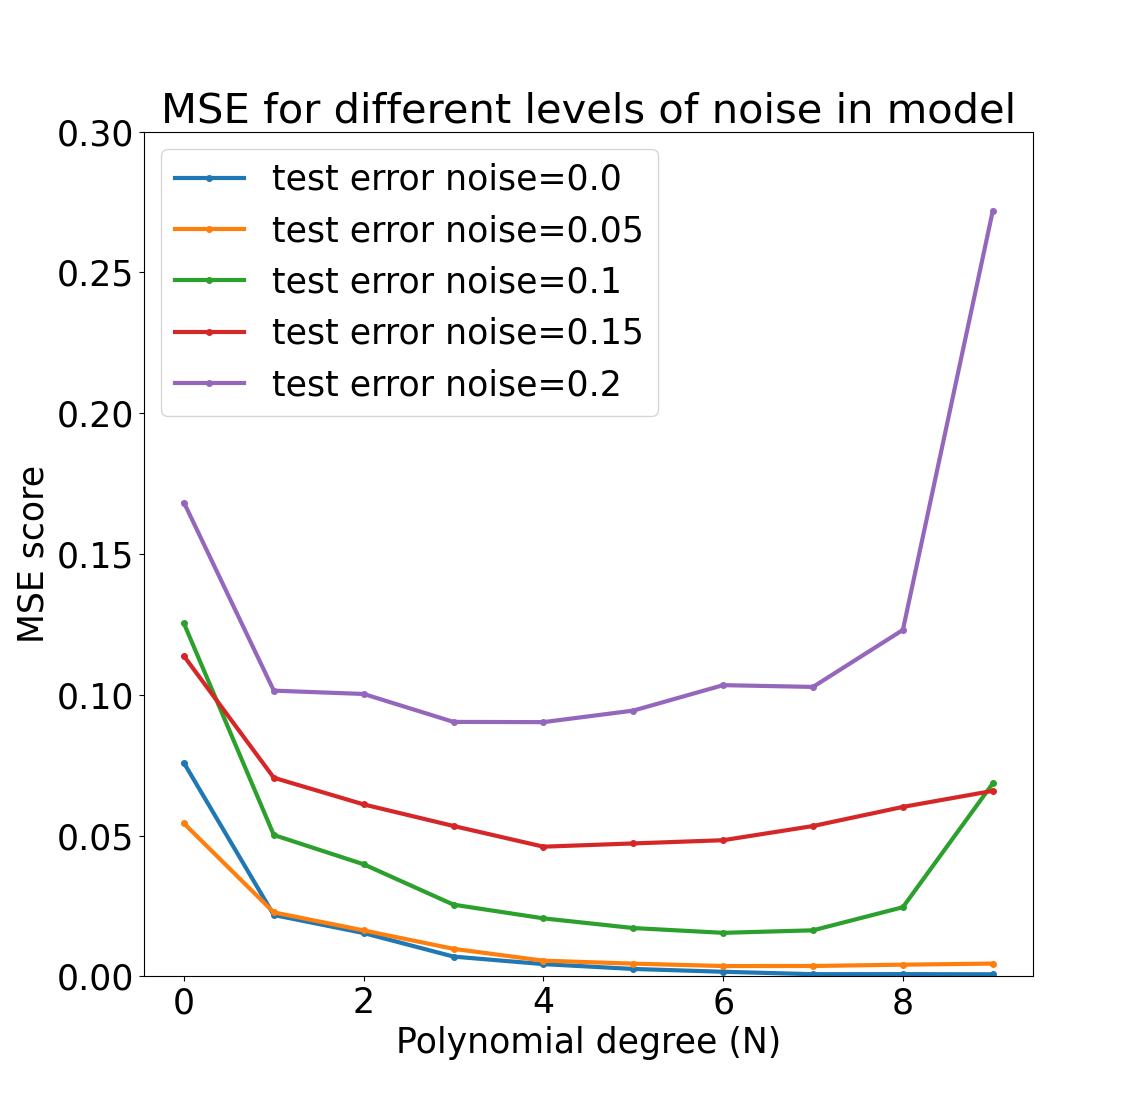
\includegraphics[width=3.25in]{figure/frankienoisecomparison.png}}
\caption{Test and train MSE for the Franke function with an increasing amount of noise}
\label{frankienoisecomparison}
\end{figure*}

\begin{figure*}
% \begin{figure}[t]
\centerline{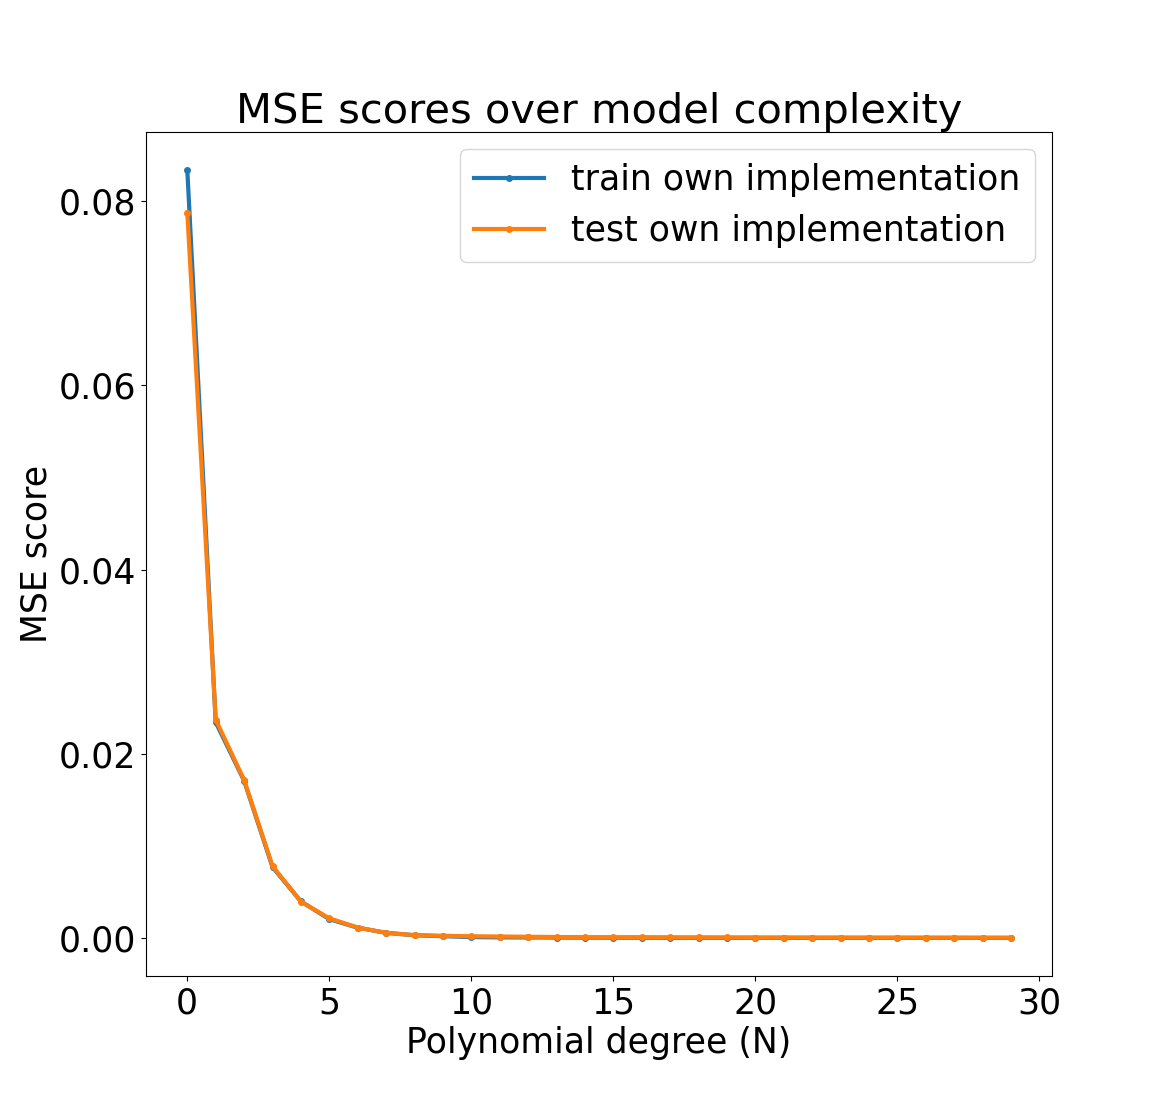
\includegraphics[width=3.25in]{figure/frankiehigherdatapoints.png}}
\caption{Franke function fitted up to polynomial degree 30, with 10000 datapoints instead of 400. As we can see, we do not overfit even at this polynomial degree when the availiable data is plentiful. The highest MSE was reached at $N=29$, and was $0.00003511$, one tenth of our best prediction with only 400 datapoints}
\label{frankiehigherdatapoints}
\end{figure*}

\end{document}
